%-----------------------------------------------%
\section{Refatoração de Software de Pesquisa}
\label{section:casesstudy:seed}

O software de pesquisa \textbf{\texttt{seed.select}} é um fork do projeto
flossSearch.Edu
... com o objetivo de ...
% Este estudo de caso é um dos resultados parciais da pesquisa de mestrado em andamento da segunda autora.


% O segundo estudo de caso foi conduzido com um grupo de pesquisa da área de Engenharia de Software e trata da ``refatoração'' de um software de pesquisa para diminuir a sua dívida técnica, social e científica.  % \texttt{seed.select}
...
\textit{Code forking} pode impactar positivamente tanto na governança quanto na sustentabilidade de projetos OSS nos níveis do software, sua comunidade e ecossistema de negócios (Nyman e Lindman, 2013).

% Entender por que os pesquisadores desenvolvem seu software e quais práticas de engenharia de software eles usam. 

\subsection{Contexto}

\subsection{Mudanças}

\begin{figure}[htb]
    \centering
    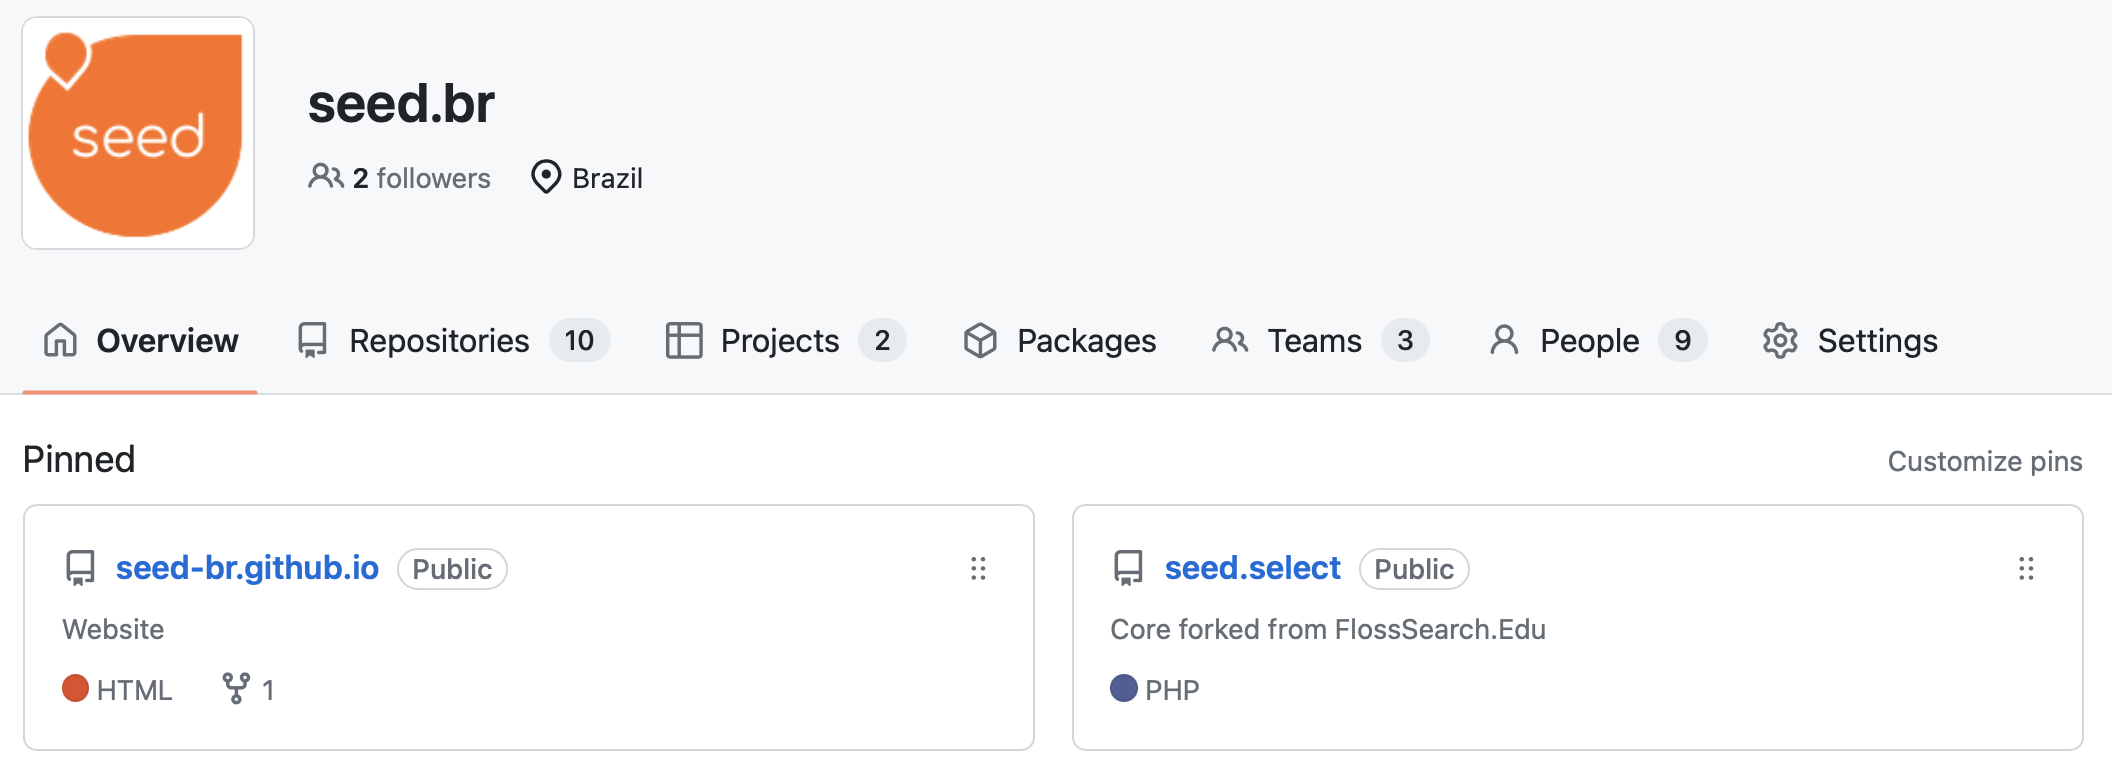
\includegraphics[scale=0.40]{JAI 2023/figures/seed-organization.png}
    \caption{Organização seed.br e repositório seed.select no GitHub.}
    \label{fig:hospedagem:seed}
\end{figure}

\noindent \textbf{\texttt{seed.select}}.
A primeiro lançamento do software ... versão 1.0.0 ...
A Figura~\ref{fig:seed-select-release} mostra ...

\begin{figure}[htb]
    \centering
    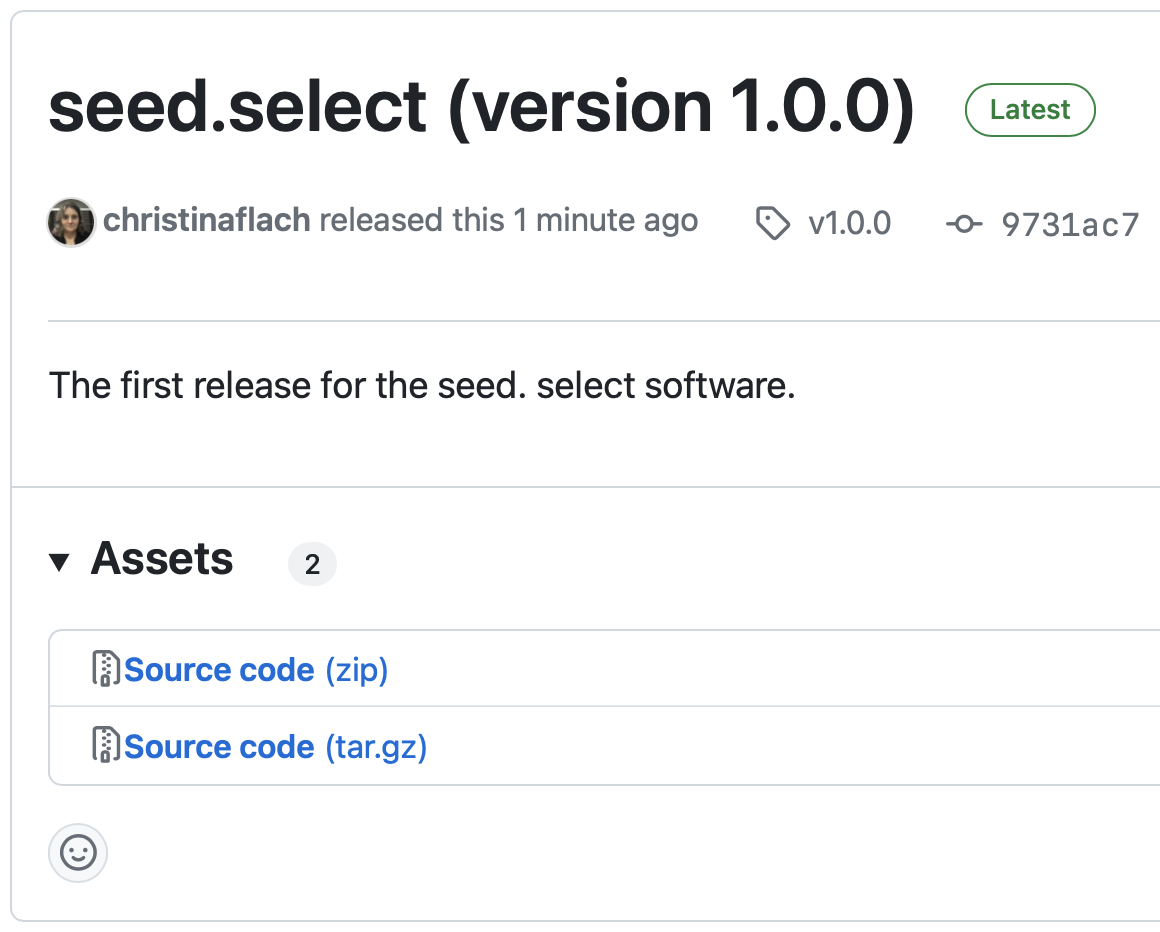
\includegraphics[scale=0.5]{JAI 2023/figures/seed-select-release-v1.0.0.png}
    \caption{Release v1.0.0}
    \label{fig:seed-select-release}
\end{figure}

\noindent \textbf{\texttt{seed.select}}.
O software não possui um PID mas possui uma versão e um identificador (URL).
Para citá-lo, atribuímos a autoria ao projeto de pesquisa no qual o software de pesquisa foi delineado e desenvolvido. 
Os nomes dos contribuidores aparecem listados no arquivo AUTHORS.md.

\begin{quote}
    SEED.BR Project (2020). seed.select (version 1.0.0) [Computer software] https://github.com/seed-br/seed.select/releases/tag/v1.0.0
\end{quote}

\noindent \textbf{\texttt{seed.select}}.
A definição de testes e uso de automação de teses foram registradas como prioritárias no kanbam do projeto.

\noindent \textbf{\texttt{seed.select}}.
O uso de ferramentas de CI/CD no desenvolvimento do
software de pesquisa X foi registrado no kanbam do projeto.

\subsection*{Avaliação da Sustentabilidade}

%\input{JAI 2023/tables/ssi-criteria-seed}

\subsection*{Avaliação de \textit{FAIRness}}

%\input{JAI 2023/tables/fairness-seed}


\subsection{Próximos passos}

\subsection{Convite para contribuir}



% The purpose of basic research is to understand and explain.
% An example within reasearch software is to understand why researchers develop they own software and which software engineering practices they use. The basic researcher has to look into the researcher (subject) thoughts and research software to find out ...